% !TEX root = ../entropy.tex

\section{Data}%
\label{sec:data}

\subsection{Data preprocessing}%
\label{sub:data_preprocessing}

Preprocessing steps
(provide detailes and links to relevant code files)
\begin{itemize}
    \item Duplicates handling.
    \item We trim all variables at the 1-percent level on the upper end of the
        distribution for variables that take non-negative values only and on
        both ends of the distribution for all other variables. We trim
        (replace outliers with missing values) rather than winsorise (replace
        outliers with the cutoff percentile value) because we believe that
        outliers result from errors in the data rather than represent genuine
        information.
    \item Actually, we don't do either of the above. With the harsher selection
        methods, the statistics are very reasonable, which, if anything, would
        suggest using winsorizing. However,
        [this](https://blogs.sas.com/content/iml/2017/02/08/winsorization-good-bad-and-ugly.html)
        article convincingly argues that we shouldn't do that in our case.
\end{itemize}

\subsection{Variable construction}%
\label{sub:variable_construction}

We classify potential determinants of savings behaviour into \textit{financial behaviours},
\textit{financial planning}, and \textit{individual or household
characteristics}, a classification frequently used in policy research on
the financial wellbeing \citep{can2019improving,cfpb2017financial, mps2018building}.

Financial behaviour

\begin{itemize}
    \item Regular savings, dummy for 10 out of last 12 months

    \item Proportion of purchases paid with credit card. This is only about 6
        percent in our final sample, whereas it is 12 percent in the full
        sample.\footnote{Across the UK, the proportion of credit pard purchases
            is about 17 percent in a typical month \citep{ukfinance2021card}.
            The proportion in our data is likely lower because the sample is
        skewed towards more affluent individuals.}

    \item Month total and category spend (category spend for robustness)
\end{itemize}

Planning
\begin{itemize}
    \item Regular login, dummy for 1 / month in 10 out of last 12 months. Have
        login data for about 50 percent of sample, so best to work with full
        sample once I use it. Implement once I can do that. -- not yet
        implemented --
\end{itemize}

Individual and household characteristics
\begin{itemize}
    \item Gender

    \item Age

    \item Urban

    \item Region

    \item Month income, winsorised at top 1 percent-level.

    \item Year income, winsorised at the 1 percent level.

    \item Regular income, dummy for 10 out of last 12 months

    \item Month income std -- not implemented yet --

    \item Income current month, dummy for month income > 0

    \item Has children, imperfect -- not yet implemented --

    \item Index of multiple deprivations from nspl -- not implemented yet --

    \item Received benefits

    \item Receives pension

    \item Housing tenure: mortgage, rent, other (owning outright implied)

    \item Takes out (payday) loan

    \item Total balance or balance / avg. month spend -- not yet implemented --
\end{itemize}







\subsection{Variabel description}%
\label{sub:variabel_description}

%todo: ggplot figure and add explanatory note
\begin{figure}[H]
    \caption{Demographic characteristics of Money Dashboard users}
    \label{fig:demographics}
    \begin{center}
        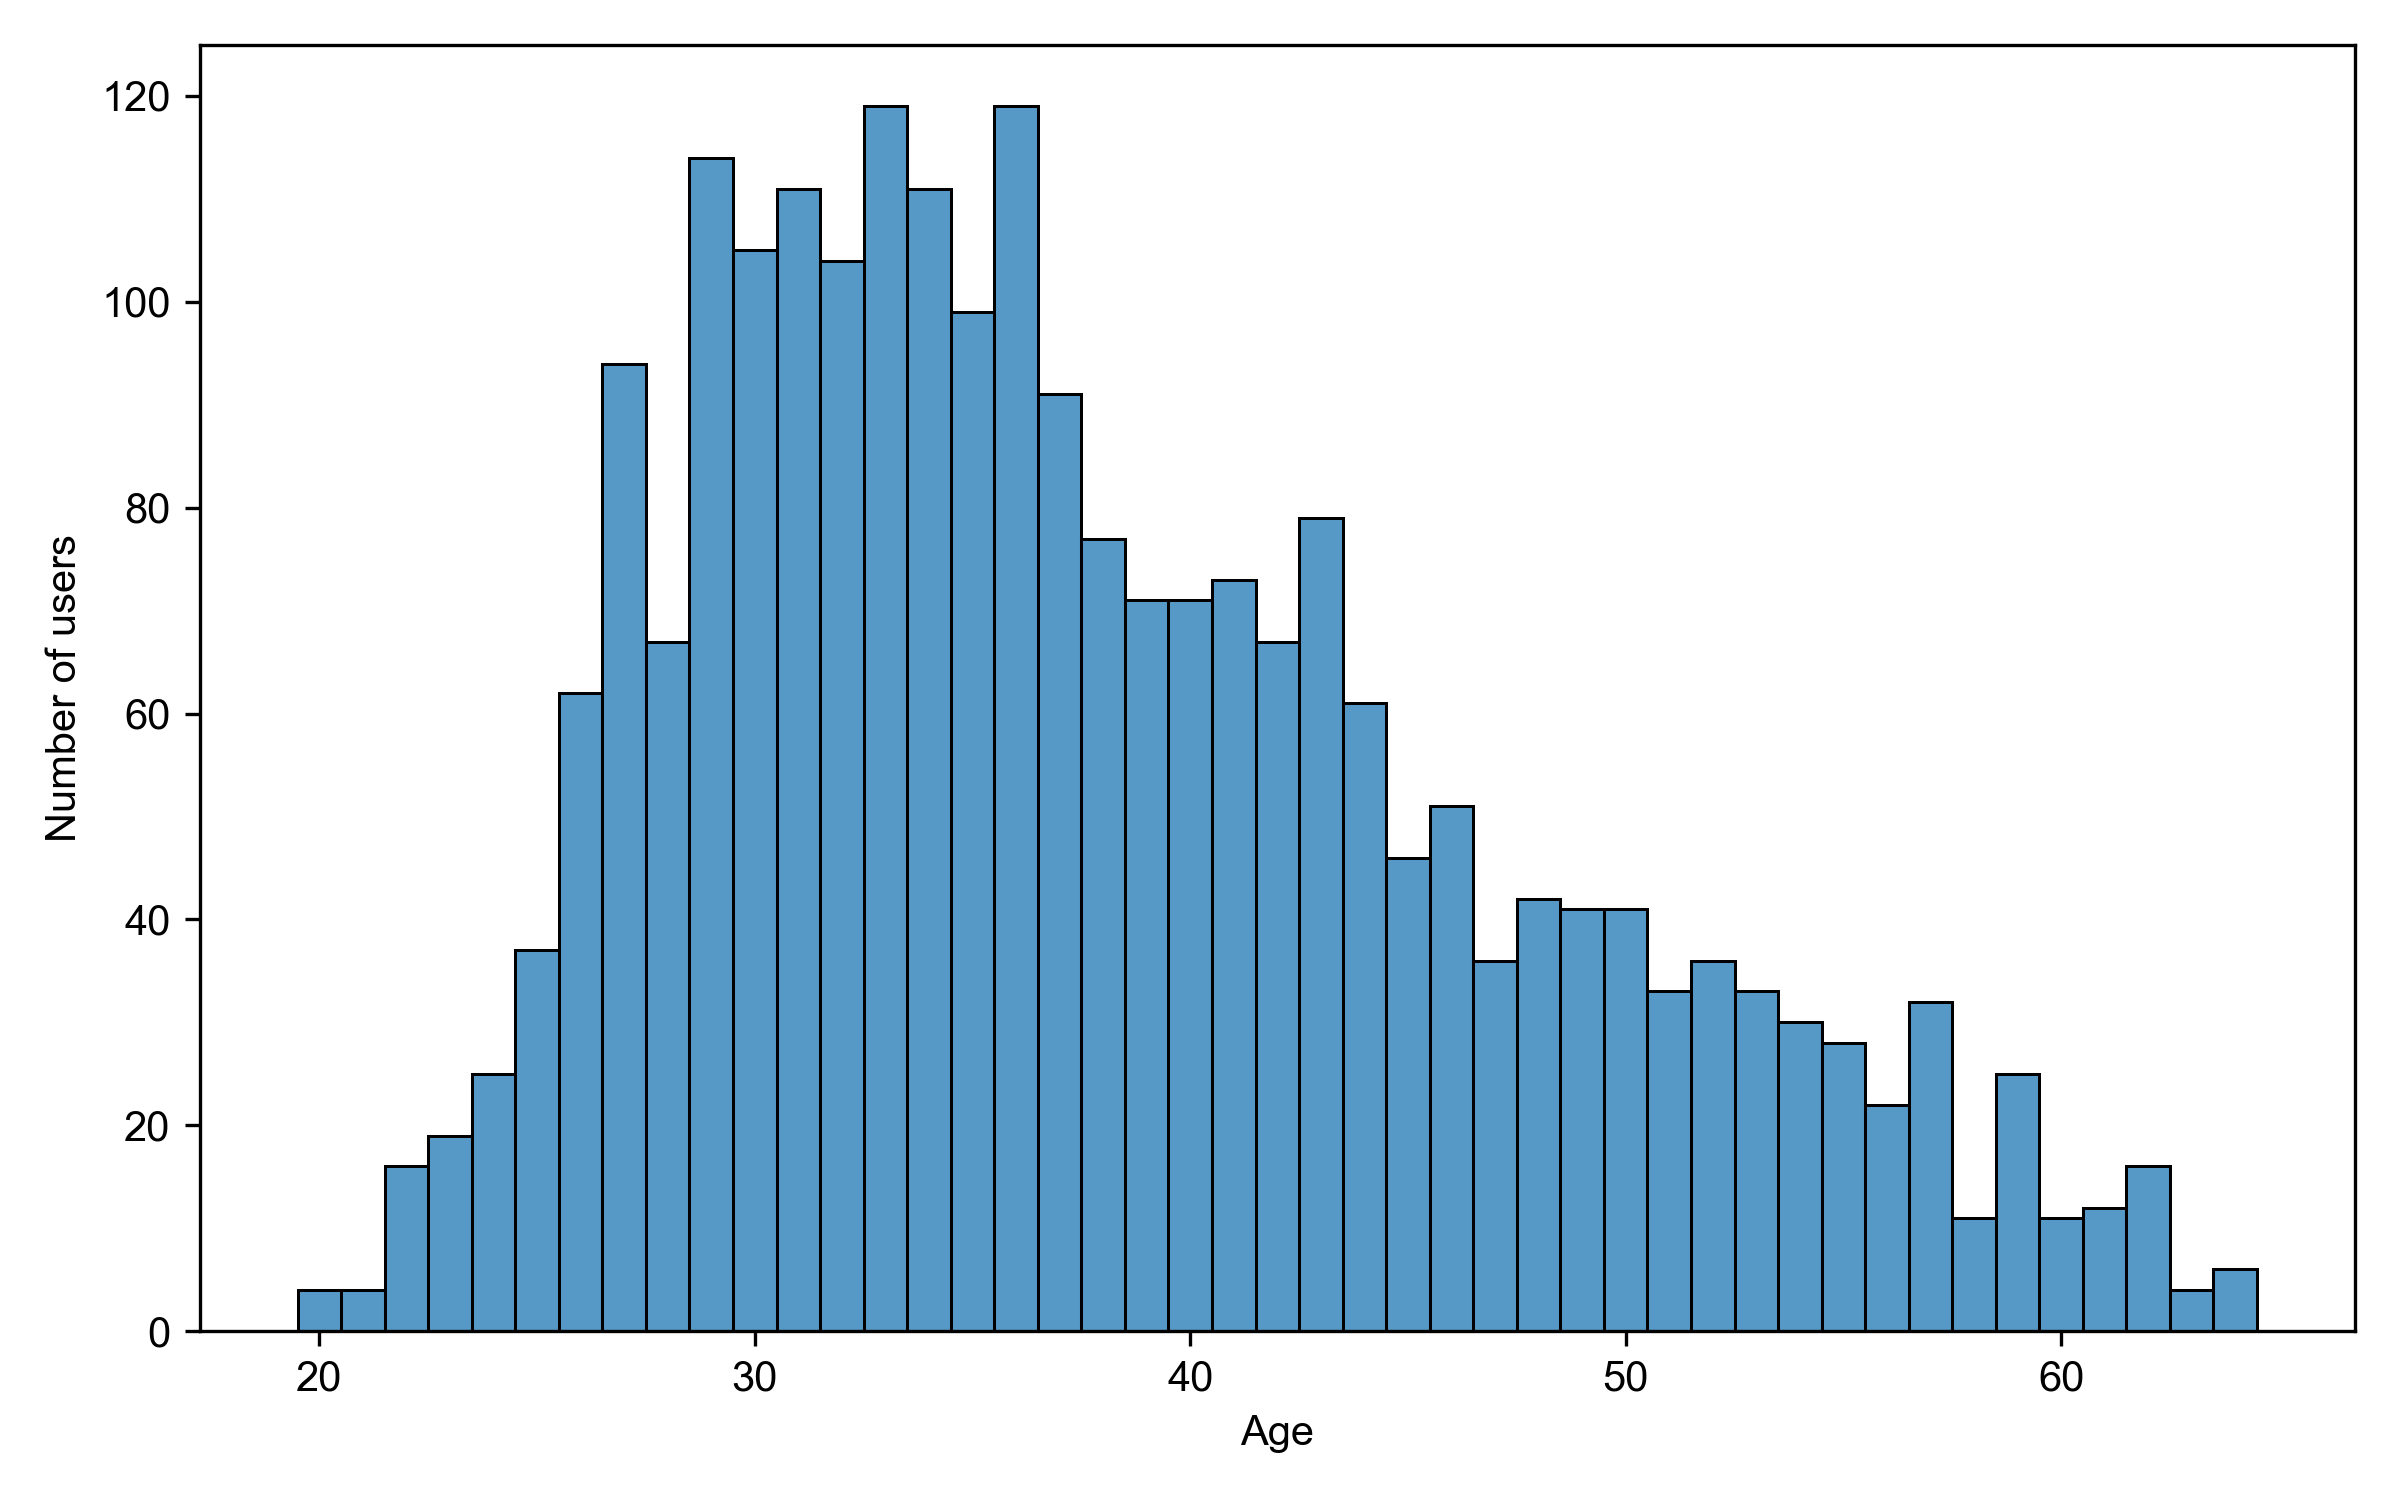
\includegraphics[width=0.49\textwidth]{\figdir/user_age_hist.png}
        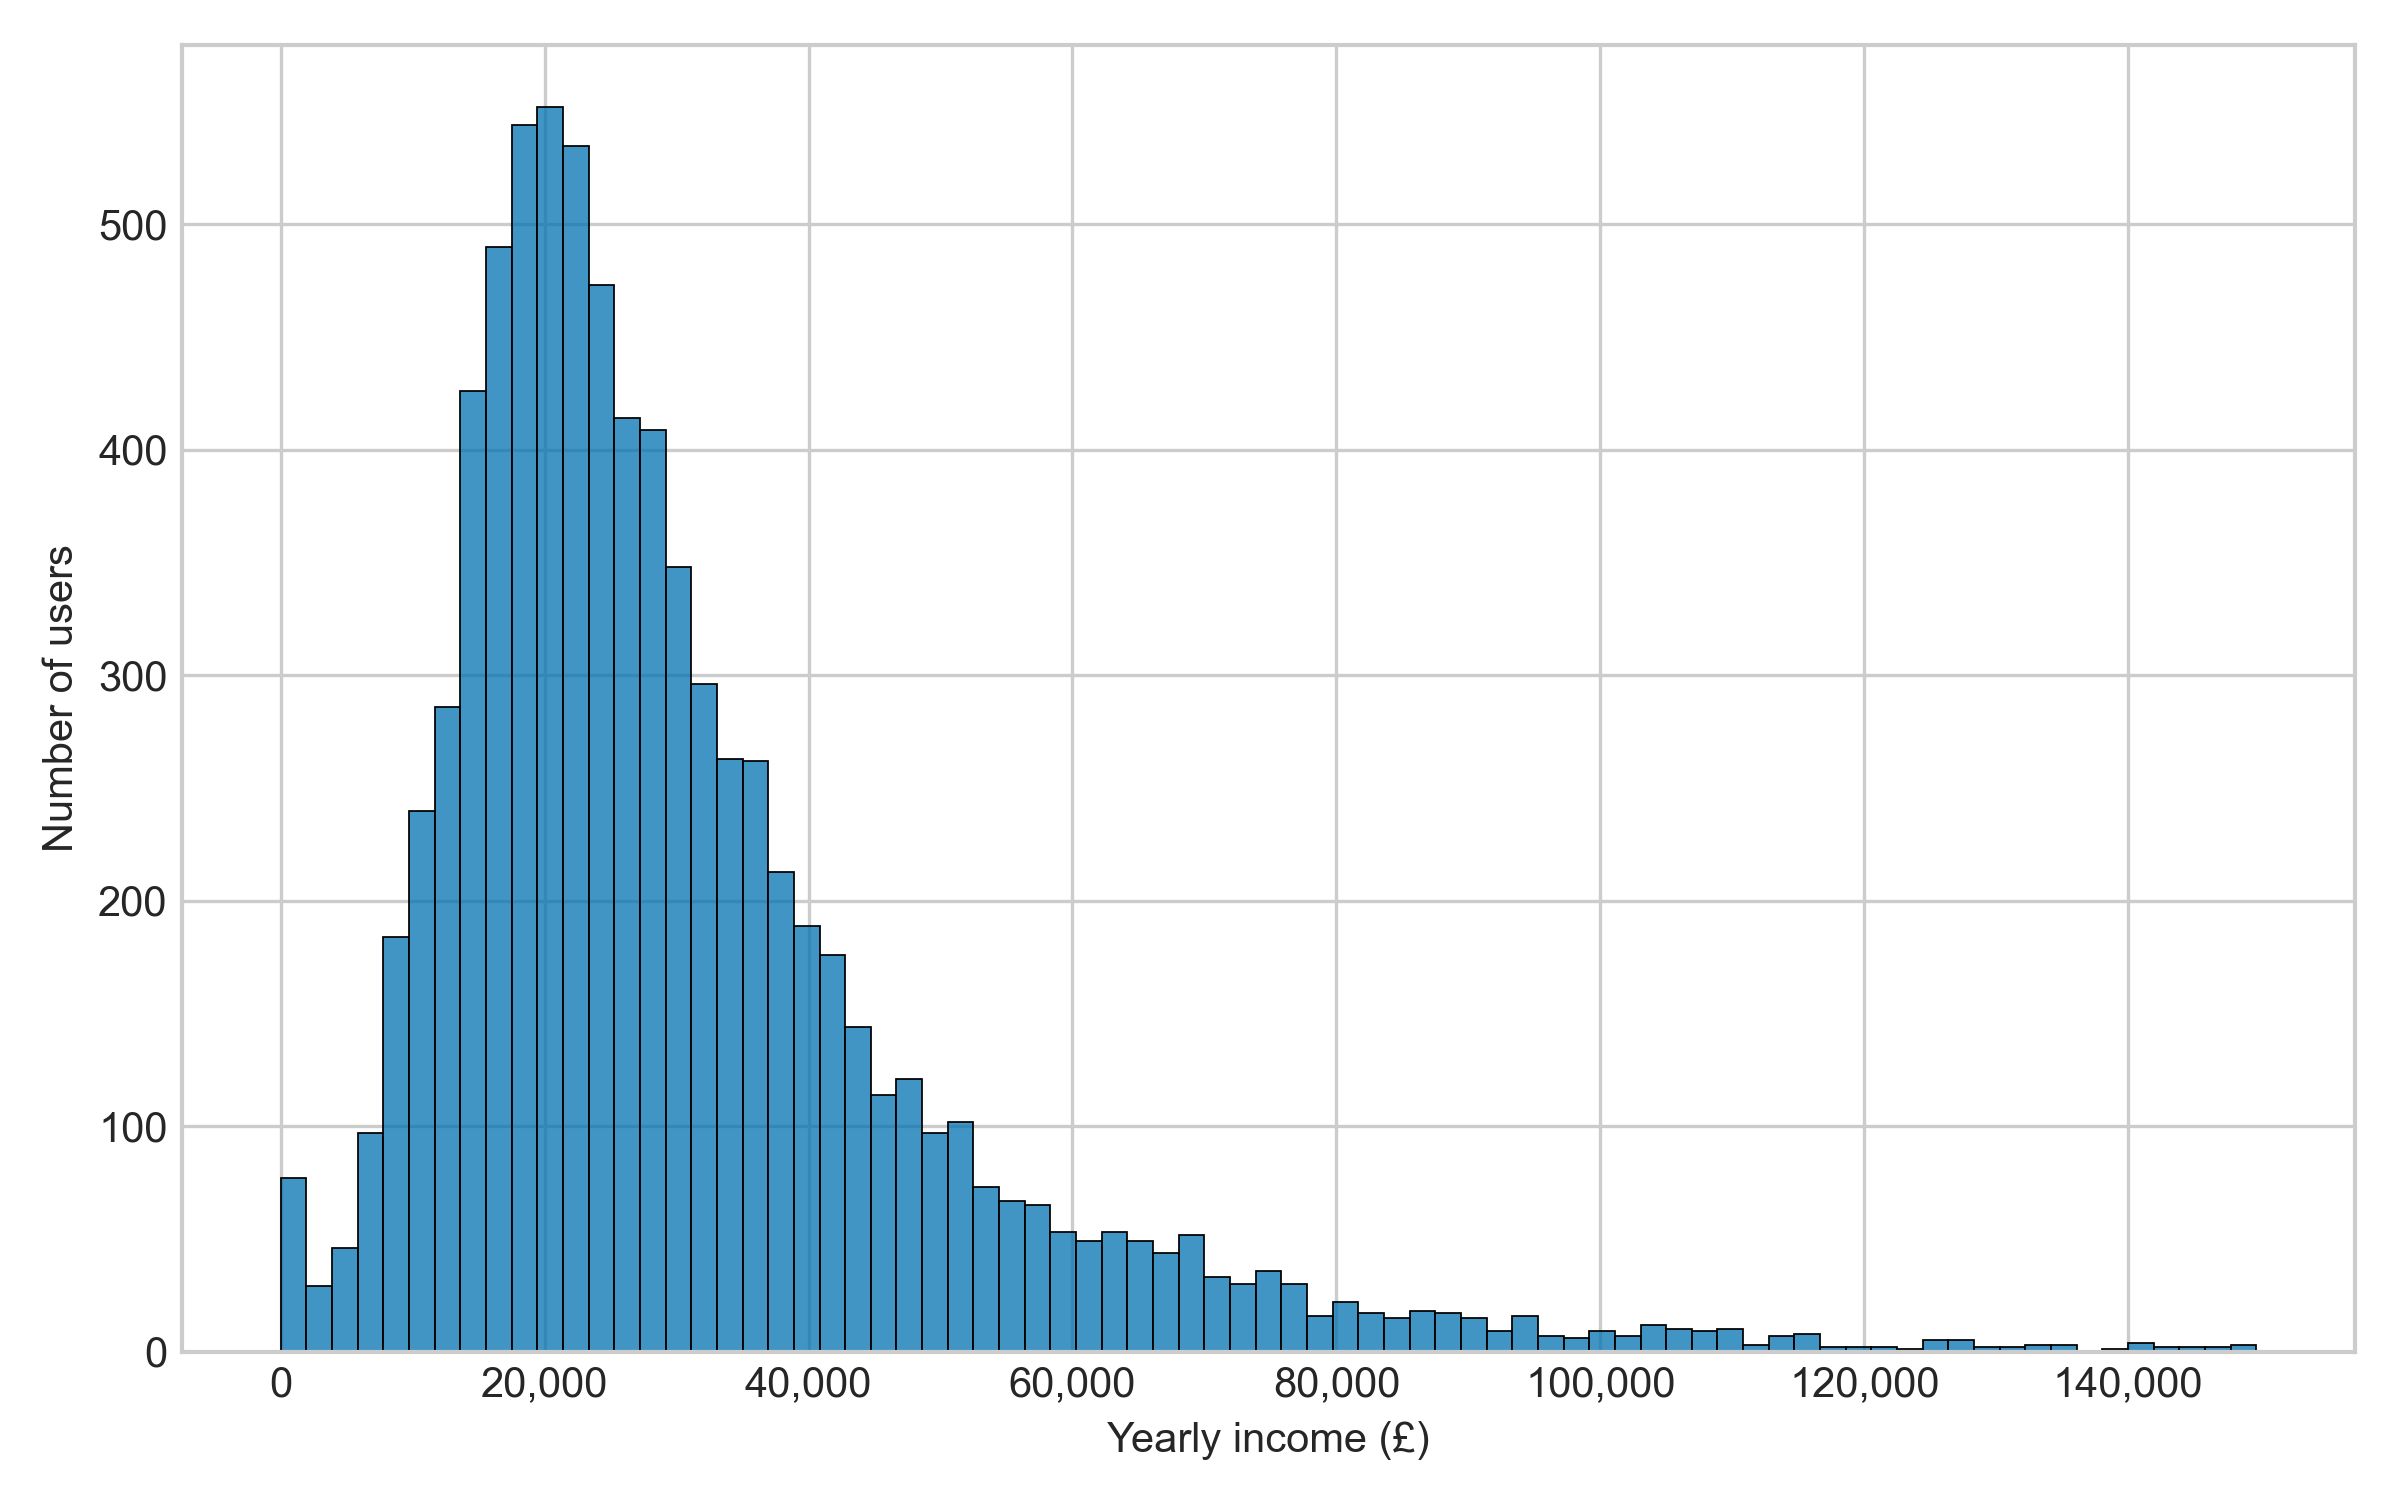
\includegraphics[width=0.49\textwidth]{\figdir/user_income_hist.png}
        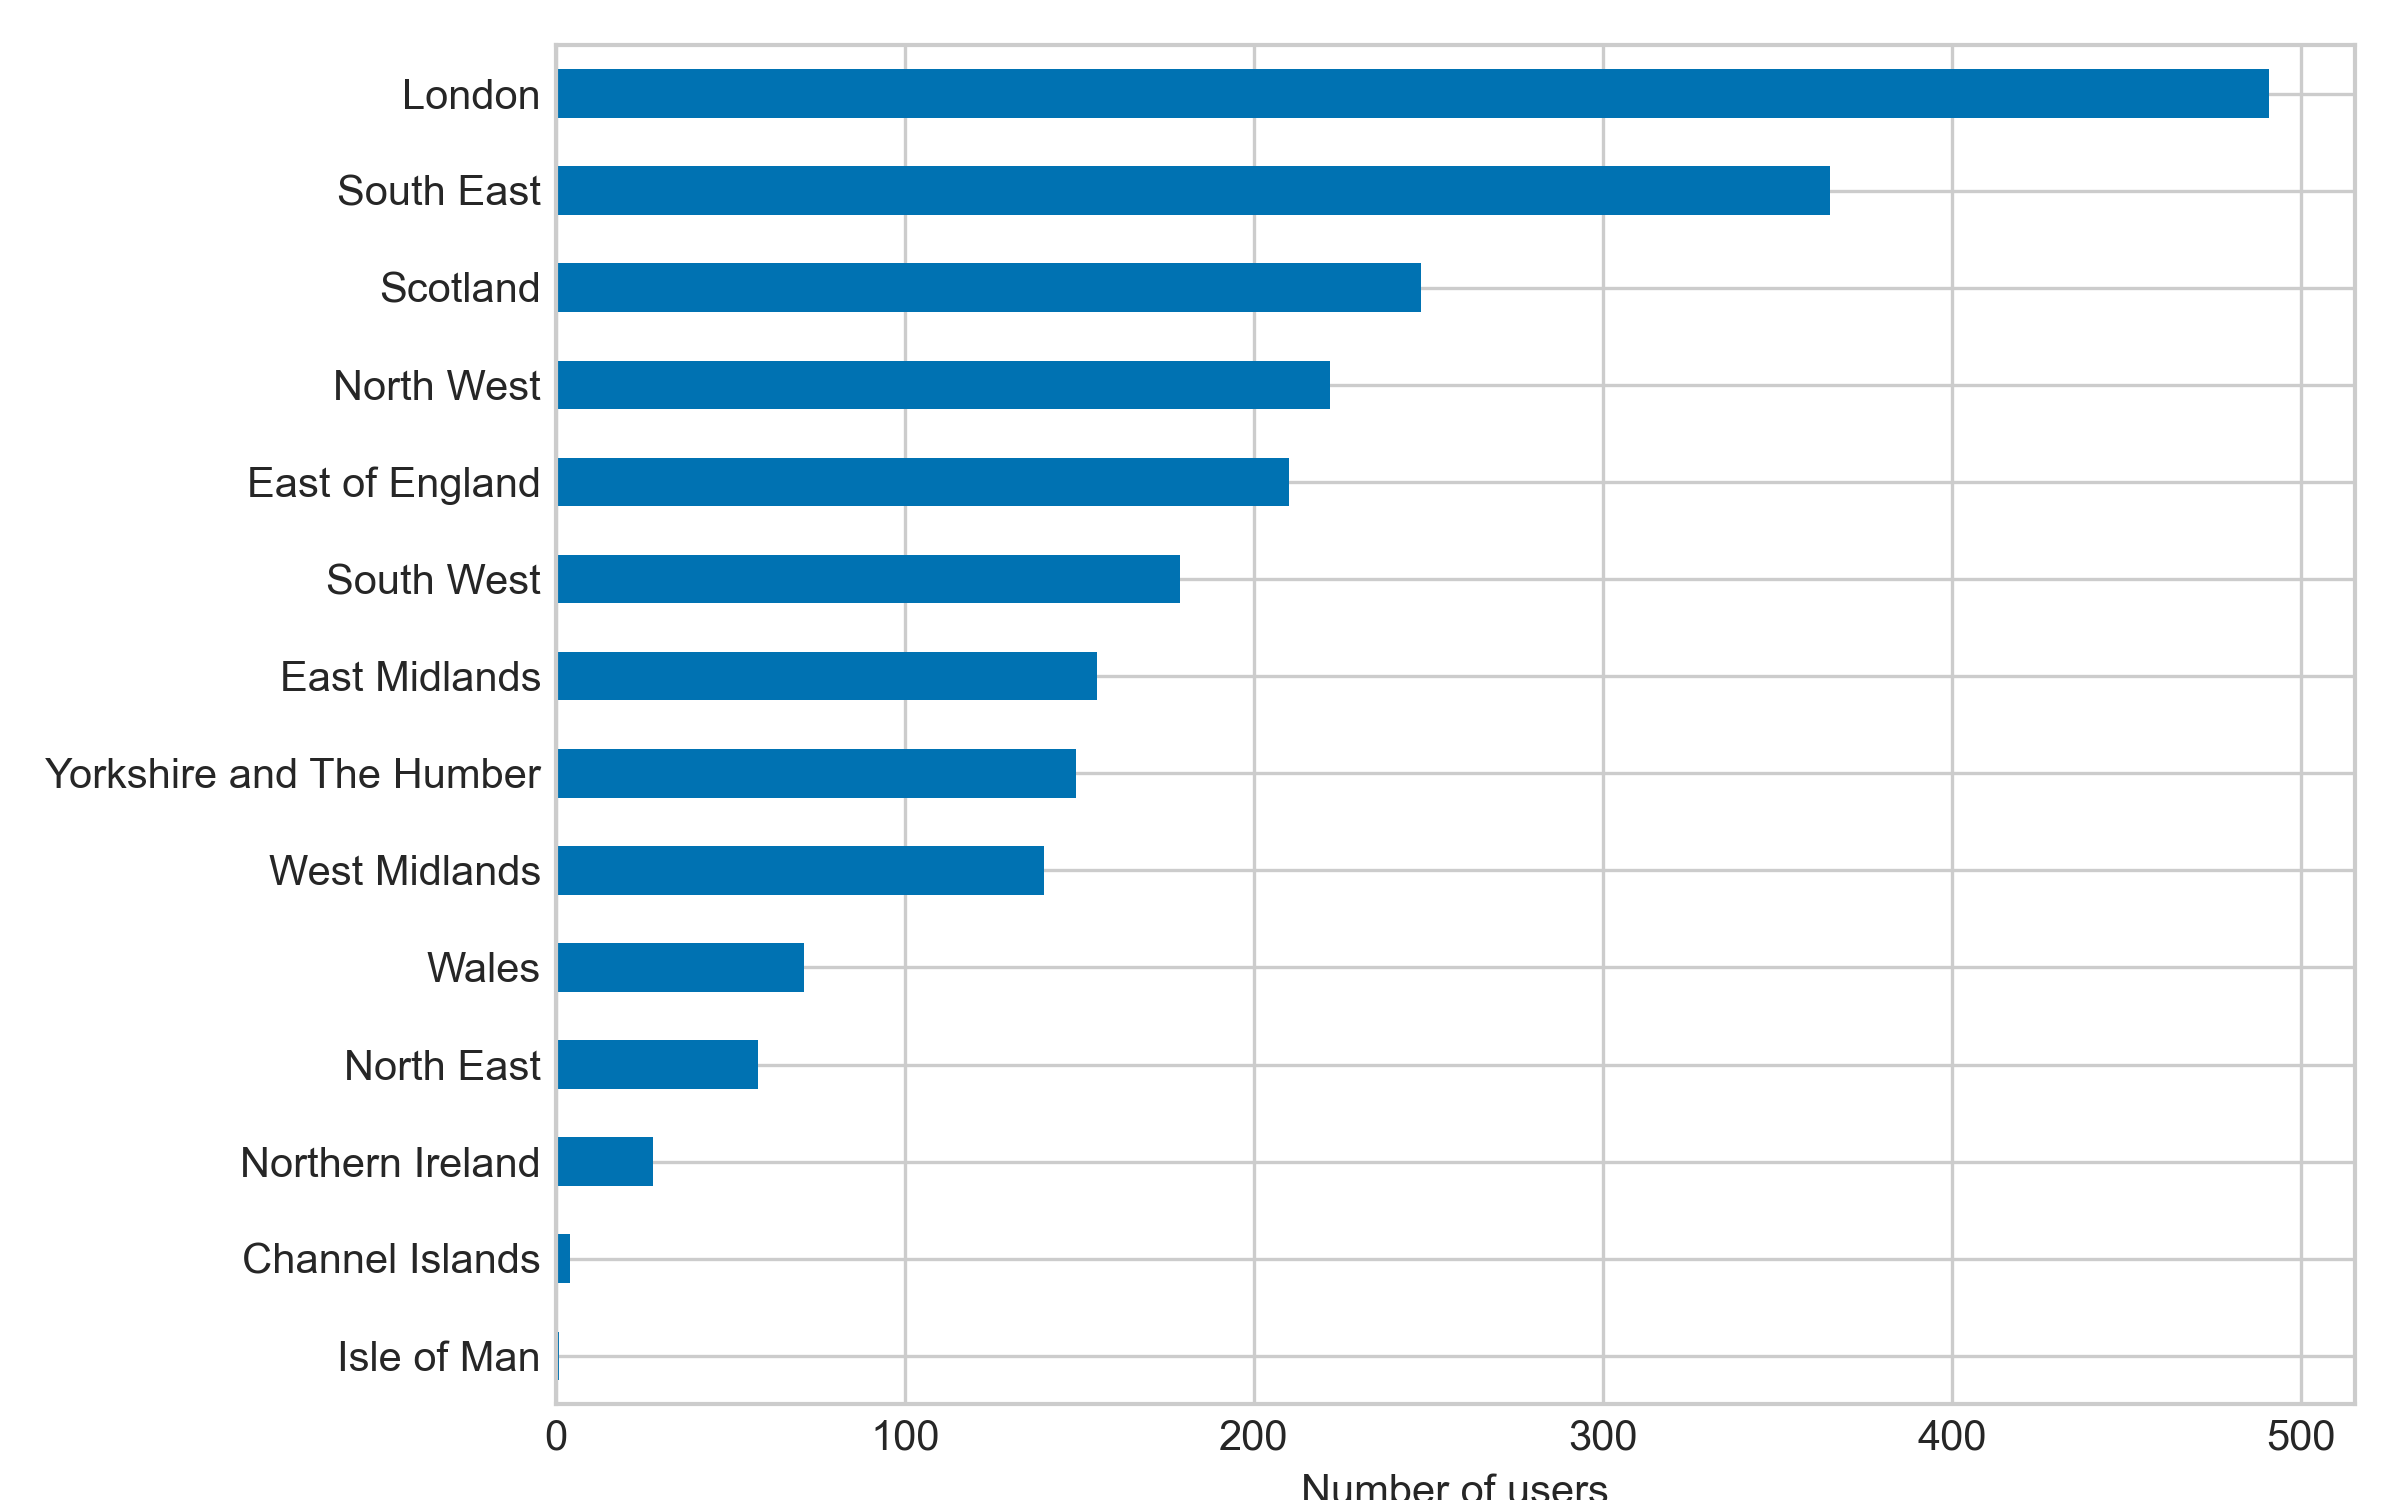
\includegraphics[width=0.49\textwidth]{\figdir/user_region_distr.png}
        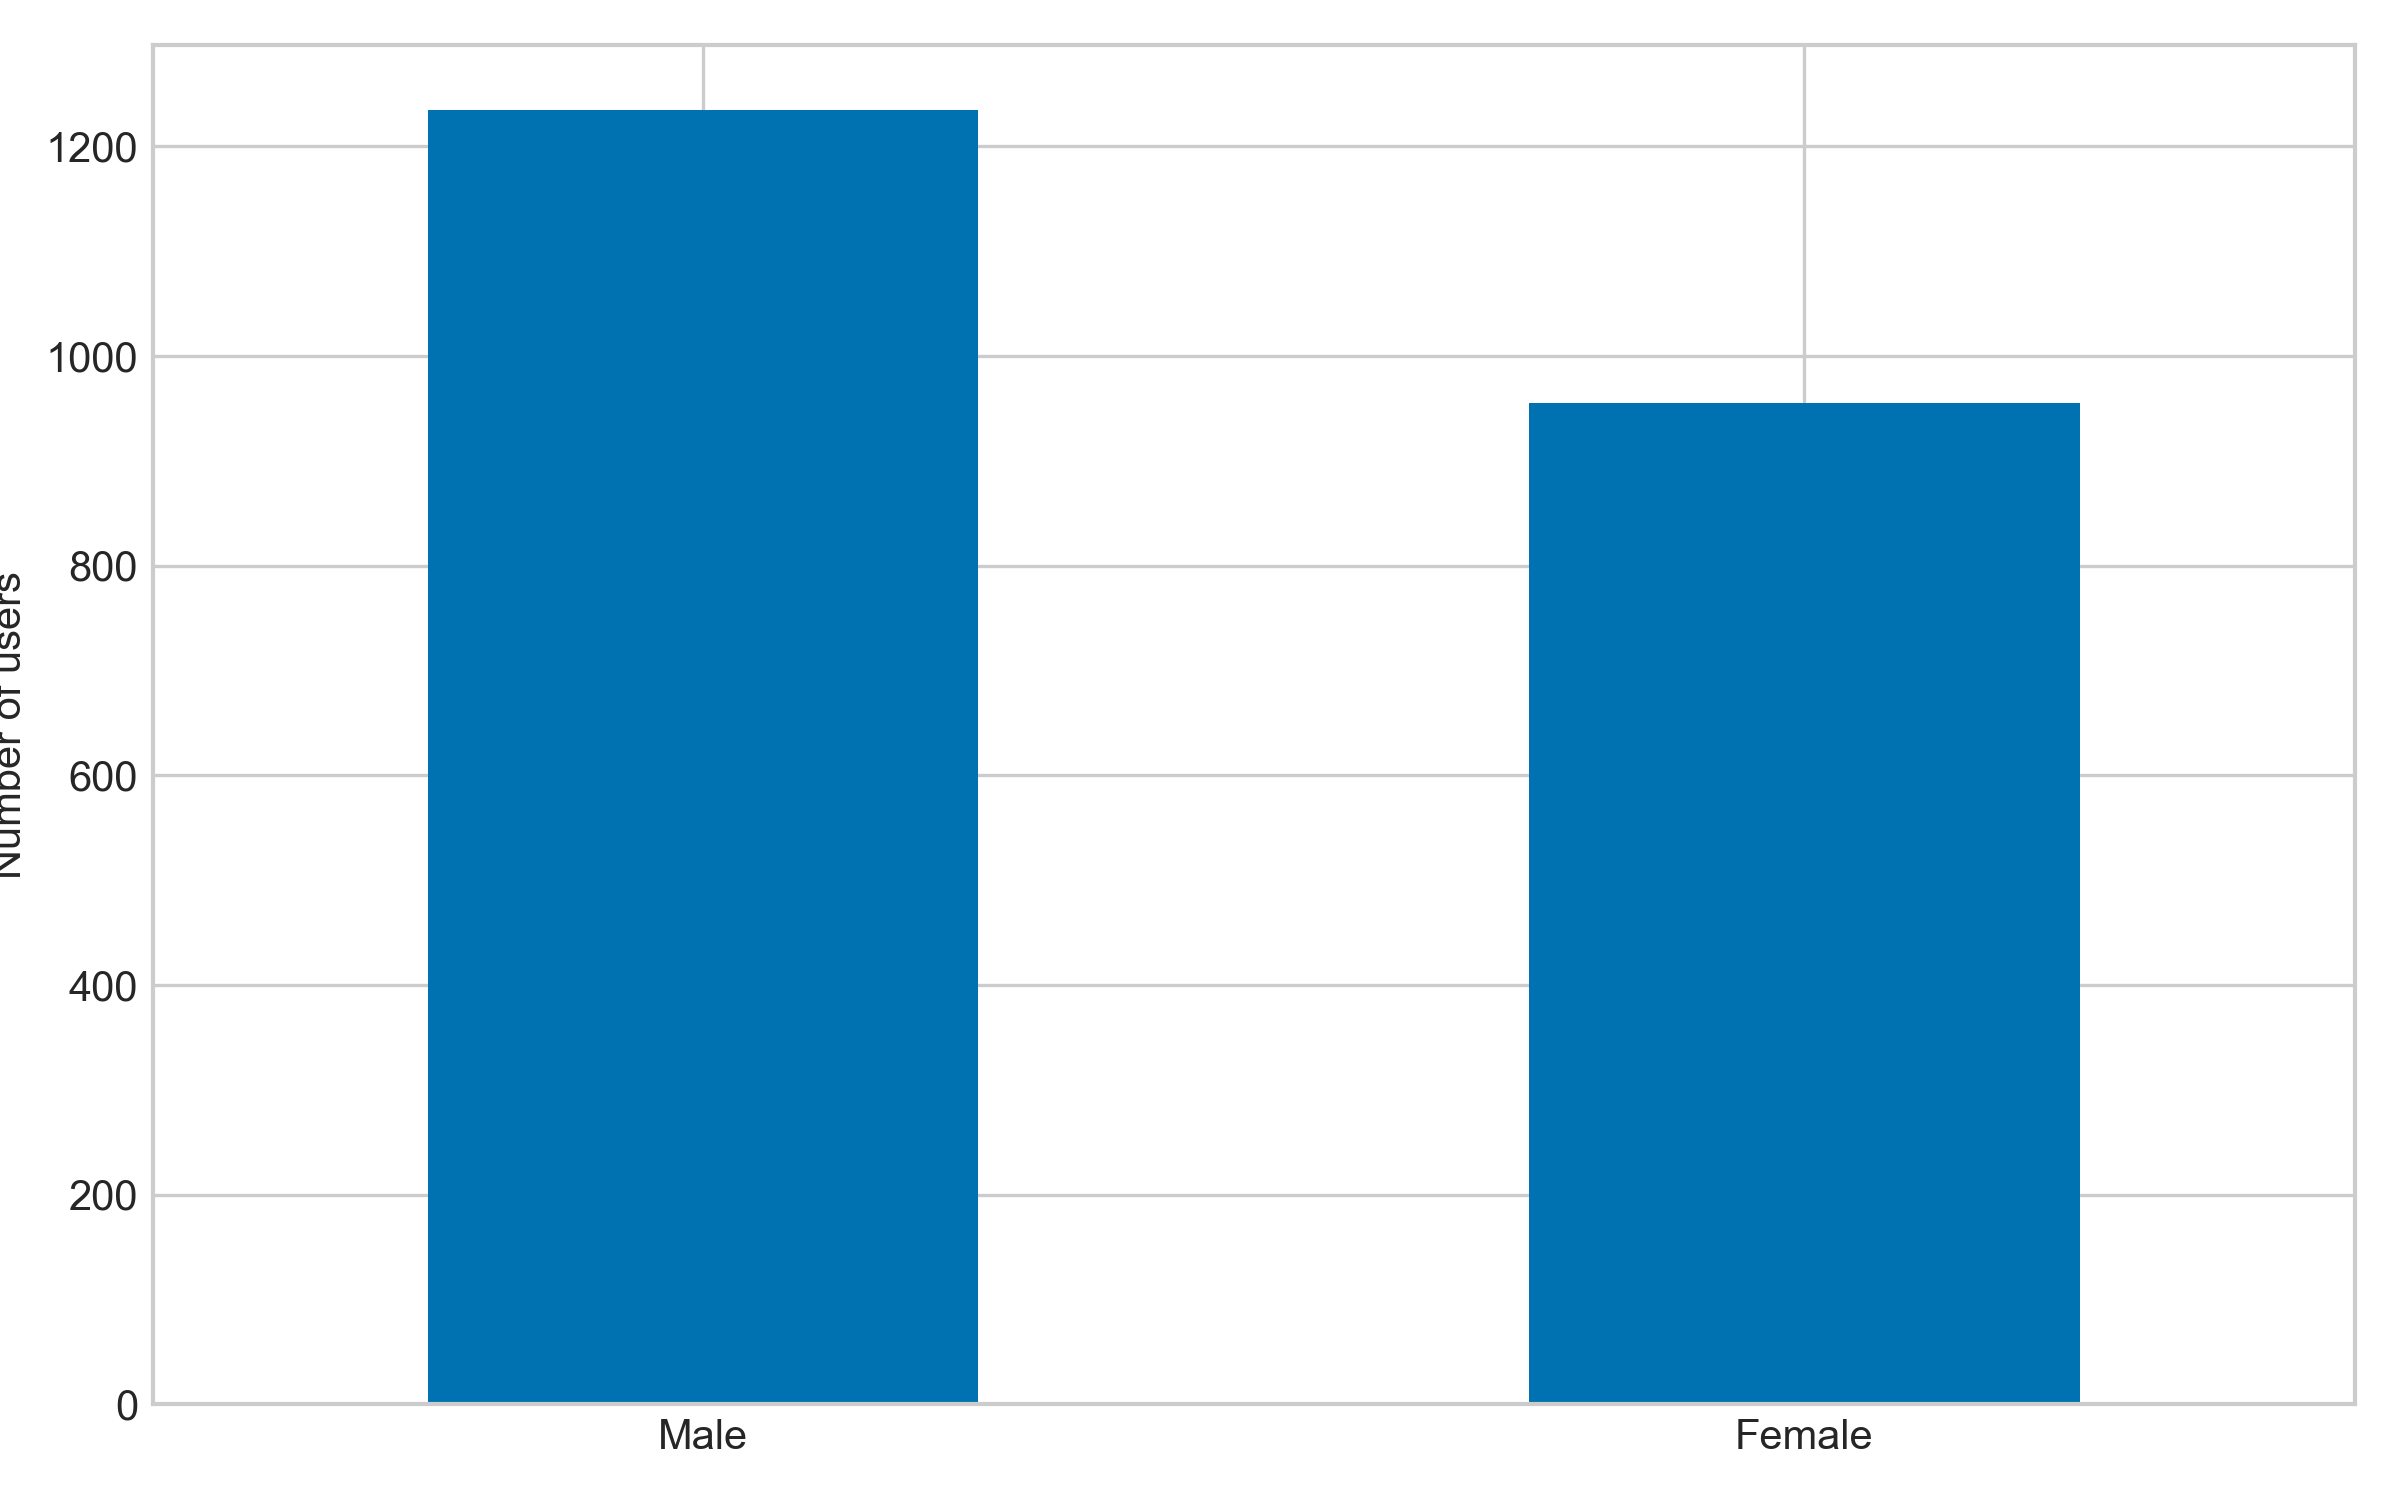
\includegraphics[width=0.49\textwidth]{\figdir/user_gender_distr.png}
    \end{center}
\end{figure}

Exploration of control variables here (e.g. like jpmorgan2019weathering for
income stability)





\subsection{Data issues}%
\label{sub:data_issues}

\citet{bourquin2020effects} argue that because some of the accounts in the data
will be joint accounts, units of observations should be tought of as
"households" rather than "users". We do not agree that this is the most prudent
approach. The validity of thinking of units as households depends on the
proportion of users in the data who add joint accounts and on the proportion of
transactions -- out of a user's total number of transactions -- additionally observed as a
result. Given that the sample is skewed towards younger individuals we think it
is unlikely that a majority of them has added joint accounts. Furthermore, it
seems reasonable to assume that in most cases, joint accounts are mainly used
for common household expenditures similar that are similar to those of a single
user (albeit in higher amounts), and are thus unlikely to alter the observed
spending profile much. Thus, we think of units of observations as individuals,
not households. 

Some accounts might be business accounts. Using versions of the algorightms
used by \citet{bourquin2020effects} to identify such accounts showed, however,
that such accounts only make up a tiny percentage of overall accounts and would
not influence our results. We thus do not exclude them.



\section{Entropy}%
\label{sec:entropy}

In equation~\ref{equ:entropy} we have defined entropy as $H =
-\sum{p_i}log(p_i)$ and pointed out that it can loosely be interpreted as the predictability of an
individual's spending behaviour. In this section, we provide a more detailed
discussion of the formula.

The building blocks of entropy is the information content of a single event.
The key intuition \citet{shannon1948mathematical} aimed to capture was that
learning of the occurrence of a low-probability event is more informative than
learning of the occurrence of a high-probability event. The information of an
event $I(E)$ is thus inversely proportional to is probability $p(E)$. One way
to capture this would be to define the information of event E as $I(E) =
\frac{1}{p(E)}$. Yet this implied that an event that is certain to occur had
information 1, when it would make sense to have information 0. To remedy this
(and also satisfy additional desireable characteristics of an information
function), we can can use the log of the expression. Hence, the information of
event E, often called \textit{Shannon information}, \textit{self-information},
or just \textit{information}, is defined as:

\begin{equation}
    I(E) = log\left(\frac{1}{p(E)}\right) = -log(p(E))
\end{equation}

Entropy, often called \textit{Information entropy}, \textit{Shannon entropy},
or just \textit{entropy}, is the information of a random variable and captures
the expected amount of information of an event drawn at random from the
probability distribution of the random variable. It is calcualted as:

\begin{equation}
    H(X) = -\sum_x p(x) \times log(p(x)) = \sum_x p(x)I(x) = \mathbb{E} I(x).
\end{equation}

% For a single event, the key intution was that the less likely an event, the
% more information is conveyed when it occurs. The related idea for distributions
% is similar: the more skewed a distribution, the more uncertain the autcome, the
% higher its entropy. The minimal entropy distribution is thus the uniform
% distribution.

\edit{todo: Discuss link to spending behaviour}
% --todo-- correct the above, it's incorrect. uniform is max entropy
% distribution. Link to spending behaviour.



% -p Why does entropy (when calculated using base 2 logarithms) also represent the number of bits required to convey the average outcome of a distribution? [Wikipedia](https://en.wikipedia.org/wiki/Entropy_&28information_theory%29#Introduction) (in the second to last paragraph of the introduction) explains this well. Basically, its because if there are some events with very high probability, then these events could be transmitted with short codes of only a few bits, so that most of the time, only a few bits have to be transmitted to send the message.

% The choice of the base for the
% logarithm varies by application and determines the units of $I(E)$. Base 2
% means that information is expressed in bits. The natural logarithm, another
% popular choice, expresses information in \textit{nats}.

\subsection{Entropy calculation}%
\label{sub:entropy_calculation}


Entropy can be calculated along a number of dimensions.

\begin{itemize}
    \item Category-based vs time-based vs category-time based
        \citep{guidotti2015behavioral, krumme2013predictability}

    \item Count-based vs value-based

    \item Intratemporal vs intertemporal \citep{krumme2013predictability}

        \begin{itemize}
            \item Based on behaviour within a given time period or changes in
                behaviour across time periods.
        \end{itemize}
        
\end{itemize}

Desireable features of entropy variable:

\begin{itemize}
    \item Based on a large enough number of categories so that spend on many of
        them can reasonably be interpreted as chaotic (the 9 LBG tags seem
        insufficient for this, especially because most of them are vital life
        expenses). Use of auto tags or merchant seems preferable.

    \item 
\end{itemize}
